
\documentclass[runningheads,a4paper]{uwsese}

%ACHTUNG: Diesen Import für englische Arbeiten entfernen.
\usepackage[ngerman]{babel}

\usepackage[utf8]{inputenc}
\usepackage{amssymb}
%\usepackage{amsmath}
\setcounter{tocdepth}{3}
\usepackage{graphicx}
\usepackage{array}
\usepackage{ragged2e}
\usepackage{arydshln}
\newcolumntype{P}[1]{>{\RaggedRight\hspace{0pt}}p{#1}}
%\newcolumntype{P}[1]{>{\raggedright\arraybackslash}p{#1}}
\usepackage{url}
\urldef{\mailsa}\path|maximilian.stock@stud-mail.uni-wuerzburg.de|
\newcommand{\keywords}[1]{\par\addvspace\baselineskip\noindent\keywordname\enspace\ignorespaces#1}

\begin{document}

\mainmatter

% first the title is needed
\title{Konfigurationsmanagementstrategien und Tools in der SW-Entwicklung:\\ Überblick und Beispiel}

% a short form should be given in case it is too long for the running head
\titlerunning{Konfigurationsmanagementstrategien und Tools}

\author{Maximilian Stock und Michael Steininger}

% \authorrunning{
%   Maximilian Stock\\
%   \texttt{maximilian.stock@stud-mail.uni-wuerzburg.de}\\
%   \and\\
%   Michael Steininger\\
%   \texttt{michael.steininger@stud-mail.uni-wuerzburg.de}
% }
% (feature abused for this document to repeat the title also on left hand pages)

% the affiliations are given next
\institute{Julius-Maximilians-Universität,
Würzburg\\
%\mailsa\\
}

\maketitle


\begin{abstract}
	Hier kommt der Abstract hin. Weglassen?
\end{abstract}


\section{Einführung}
Ursprünglich ist die Idee des Konfigurationsmanagements im US-Militär
entstanden. Dort wurden in den 1950er Jahren Versuche mit Flugkörpern gemacht,
die in verschiedenen Konfigurationen gebaut und getestet wurden. Eine
Vielzahl der Flugkörper explodierten nicht wie vorgesehen im Ziel, sondern
meist zuvor. Es war allerdings nicht möglich die fehlerhaften Flugkörper nach
den Tests zu untersuchen, weil sie zerstört wurden. Zusätzlich waren die
Aufzeichnungen über die Konfigurationen der einzelnen Flugkörper nicht
ausreichend. Dadurch war es nicht möglich festzustellen welche Änderungen zu
welchen Testausgängen führten. Aus diesen Erfahrungen enstanden
Konfigurationsmanagementstandards, die bei allen Änderungen eines Erzeugnisses
auch eine Änderung der Dokumente fordern.

Diese Probleme lassen sich analog auch in der Softwareentwicklung beobachten.
Es gibt z. B. Probleme durch undokumentierte Änderungen von Code oder
kurzfristige Änderungen am Quellcode vor Auslieferung. Deshalb ist das
Konfigurationsmanagement insbesondere in der
Automobilbranche Teil von Reifegradmodellen wie z. B. {\em CMMI} oder
{\em SPICE}. Damit überprüfen Automobilhersteller, ob ihre Zulieferer über ein
funktionierendes Konfigurationsmanagement verfügen~\cite[S. 2f]{weischedel2002}.

Zunächst wird im ersten Kapitel dieser Arbeit auf die Grundlagen des
Konfigurationsmanagement eingegangen. D. h. das Konfigurationsmanagement wird
definiert und erklärt.
Das zweite Kapitel erläutert wie man das allgemeine Konfigurationsmanagement in
der Softwareentwicklung anwendet.
In Kapitel drei wird das Konfigurationsmanagement an einem beispielhaften
Softwareprojekt in der Praxis gezeigt.

TODO: AUFBAU DER ARBEIT VOR ABGABE NOCHMAL ÜBERPRÜFEN OB ES NOCH PASST!!!!

\section{Grundlagen des Konfigurationsmanagement}
Im Folgenden wird Konfigurationsmanagement nach DIN EN ISO 10007 definiert und
dessen Tätigkeiten beschrieben. Es existieren eine Reihe von weiteren
Definitionen für Konfigurationsmanagement.
In dieser Arbeit wird im Folgenden die ISO Definition verwendet. Eine weitere
Definition ist z. B. im Buch ``Configuration Management Principles and
Practice'' von Hass beschrieben~\cite{Hass:2003:CMP:582584}. In den nächsten
Unterkapiteln werden die einzelnen Tätigkeiten des Konfigurationsmanagements
nach DIN EN ISO 10007 näher erläutert. Daraufhin folgt ein Unterkapitel über
Konfigurationsmanagementpläne.

Nach der Norm DIN EN ISO 10007 ist das Konfigurationsmanagement (kurz {\em KM})
wie folgt definiert:

``KM ist eine Managementdisziplin, die über die gesamte Lebensdauer eines
Erzeugnisses angewandt wird, um Transparenz und Überwachung seiner funktionellen
und physischen Merkmale sicherzustellen. Hauptziel von KM ist, die
gegenwärtige Konfiguration eines Erzeugnisses sowie den Stand der Erfüllung
seiner physischen und funktionellen Forderungen zu dokumentieren und volle
Transparenz herzustellen. Ein weiteres Ziel ist, dass jeder am Projekt
Mitwirkende zu jeder Zeit des Erzeugnislebenslaufs die richtige und zutreffende
Dokumentation verwendet. Der KM Prozess umfasst die folgenden integrierten
Tätigkeiten:

\begin{itemize}
	\item Konfigurationsidentifizierung
	\item Konfigurationsüberwachung
	\item Konfigurationsbuchführung
	\item Konfigurationsauditierung''~\cite{ISO10007}.
\end{itemize}

\subsection{Konfigurationsidentifizierung}
Bei der Konfigurationsidentifizierung geht es darum sog.
{\em Konfigurationseinheiten} festzulegen und zu beschreiben. Eine
Konfigurationseinheit kann dabei eine beliebige Kombination von Hardware,
Software und Dienstleistung sein. Für diese Einheiten werden in
Konfigurationsdokumenten die physischen und funktionellen Merkmale festgehalten.
Weiterhin wird bei der Konfigurationsidentifizierung festgelegt, nach welchen
Regeln bestimmte Artefakte nummeriert werden. Hier können Artefakte z. B.
Konfigurationseinheiten, ihre Teile und Zusammenstellungen von Dokumenten,
Schnittstellen und Änderungen sein. Außerdem werden sog.
{\em Bezugskonfigurationen} definiert. Diese sind mitsamt ihren Änderungen als
aktuell gültige Konfigurationen zu verstehen~\cite[S. 6f]{weischedel2002}.

\subsection{Konfigurationsüberwachung}
Die Konfigurationsüberwachung behandelt die Überwachung von Änderungen. Dabei
wird gefordert, dass alle Änderungen dokumentiert und begründet werden.
Zusätzlich sollten die Auswirkungen der Änderungen beurteilt werden. Auf Basis
dieser Beurteilungen sollen Änderungen genehmigt oder abgelehnt
werden~\cite[S. 7]{weischedel2002}.

\subsection{Konfigurationsbuchführung}
Die Tätigkeit Konfigurationsbuchführung sorgt für eine Rückverfolgbarkeit von
Änderungen. Damit soll es möglich sein, alle Änderungen zur letzten
Bezugskonfiguration nachvollziehen zu können. Aus der
Konfigurationsidentifizierung und der Konfigurationsüberwachung resultieren
die für die Buchführung notwendigen Aufzeichnungen als
Nebenprodukte~\cite[S. 7]{weischedel2002}.

\subsection{Konfigurationsauditierung}
Die Konfigurationsauditierung lässt sich in zwei Tätigkeiten aufteilen.

Durch das sog. {\em funktionsbezogene Konfigurationsaudit} wird gewährleistet,
dass das Erzeugnis den vertraglich spezifizierten Anforderungen entspricht.
D. h. die Konfigurationseinheit muss alle Leistungen und funktionellen Merkmalen
erreichen, die zuvor in den Konfigurationsdokumenten festgelegt wurden.

Das sog. {\em physische Konfigurationsaudit} prüft, ob eine aktuelle
Konfiguration einer Konfigurationseinheit mit den Konfigurationsdokumenten
übereinstimmt. Damit soll sichergestellt werden, dass die Dokumente und die
Erzeugnisse nicht voneinander abweichen gehen. Ansonsten könnte passieren, dass
ein Erzeugnis letztendlich nichts mehr mit seiner Dokumentation zu tun
hat~\cite[S. 7]{weischedel2002}.

\subsection{Konfigurationsmanagementplan}
Der Konfigurationsmanagementprozess sollte in einem
{\em Konfigurationsmanagementplan} dokumentiert sein. Darin sollte für jedes
Projekt stehen welche Konfigurationsmanagementverfahren durchzuführen sind. Zu
jedem Verfahren soll im Plan festgelegt sein wer sie durchführt und wann sie
ausgeführt werden sollen~\cite[S. 7f]{weischedel2002}.

TODO: "Ein Beispiel für einen Konfigurationsmanagementplan ist in X zu sehen"

\section{Konfigurationsmanagement für Softwareentwicklung}

Konfigurationsmanagement lässt sich ebenfalls in der Softwareentwicklung
unter der Bezeichnung {\em software configuration management} (kurz SCM)
finden. Nach Pressman \cite[p. 585f]{Pressman:2009:SEP:1593949} besteht eine
Softwarekonfiguration aus Einzelteilen, die zu mindestens einer der folgenden
drei Kategorien gehören:

\begin{quote}
  The output of the software process is information that may be divided into three
  broad categories: (1) computer programs (both source level and executable forms),
  (2) work products that describe the computer programs (targeted at various
  stakeholders), and (3) data or content (contained within the program or external
  to it).
\end{quote}

Zur zweiten Kategorie zählen hierbei z. B. jegliche Dokumente die das Softwaresystem
spezifizieren (Anforderungsdokument, Architekturdokument, Testspezifikationen, etc.).
Mit der dritten Kategorie sind zusätzliche Inhalte gemeint, die zu einem gewissen
Grad mit der Software zu tun haben. Beispiele hierfür sind Konfigurationsdateien
für das korrekte Ausführen der Software auf dem Zielsystem, Konfigurationen für
verwendete Test-/Build-/Deploysoftware, Compiler in bestimmten Versionen, etc.
Systembestandteile die in eine dieser Kategorien fallen heißen
{\em software configuration items} (kurz SCI) und bilden zusammen die eine
{\em software configuration} (kurz SC).

Im Prozess der Softwareentwicklung enstehen zwangsläufig gänzlich neue SCIs oder
Abwandlungen von bestehenden.
Innerhalb dieses Prozesses beschreibt SCM eine Menge von Schritten um die
Veränderungen der SCIs zu handhaben. Derartige Änderungen entstehen in
der Regel durch folgende Gründe:

\begin{itemize}
	\item Businessregeln or Produktanforderungen ändern sich aufgrund neuer Marktbedingungen
	\item Stakeholder fordert Modifikationen am System um zusätzliche Informationen/Dienste
        oder mehr Funktionalität zu bieten
	\item Prioritäten des Projekts oder die Struktur im Projektteam ändert sich
	\item Zeitliche oder finanzielle Planung erfordert Neuplanung des Projekts
\end{itemize}





% IRRELEVANT?!
% \subsection{Baselines}
% Da im Kontext des SCM und der enstehenden SCIs der Begriff der baselines auftritt,
% wird er im Folgenden definiert.
% Innerhalb des Lebenszyklus eines Projektes werden sogenannte {\em baselines}
% verwendet, um konkrete Softwarekonfigurationen in Meilensteinen festzuhalten.
% Die IEEE definiert den Begriff folgendermaßen \cite[p. 588]{Pressman:2009:SEP:1593949}:
%
% \begin{quote}
%   A specification or product that has been formally reviewed and agreed upon,
%   that thereafter serves as the basis for further development, and that can be
%   changed only through formal change control procedures.
% \end{quote}
%
% Damit ist eine baseline ein konkreter Stand aller SCIs, der formal anerkannt
% wird um diesen hervorzuheben. Dies kann z. B. der Fall sein, sobald eine bestimmte
% Funktionalität durch das Produkt angeboten wird. Durch die Einführung von baselines
% können Fortschritte besser festgehalten werden.

\subsection{SCM Repository}
Unter einem {\em SCM repository} versteht man eine Menge von Mechanismen und
Datenstrukturen um auftretende Änderungen im Softwareentwicklungsprozess
effektiv zu verwalten. Es bietet Funktionalitäten eines modernen Datenbanksystems,
da es z. B. die Datenintegrität der zu speichernen SCIs garantieren muss.
Außerdem stellt es einen zentralen Baustein im Entwicklungsprozess dar, unterstützt
bei der Qualitätssicherung und bietet Integrationen für externe Softwarewerkzeuge
\cite[p. 590f]{Pressman:2009:SEP:1593949}. Abbildung \ref{fig:scm_repository_content}
zeigt welche Inhalte in der Regel in einem SCM-Repository enthalten sind.

\begin{figure}
%\vspace{-2mm}
\begin{center}
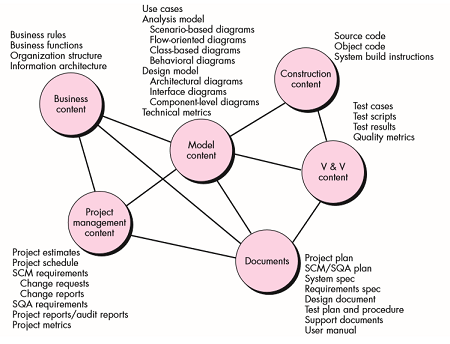
\includegraphics{graphics/scm_respository_content.png}
\caption{Inhalte eines SCM-Repositories nach Pressman
\cite[p. 591]{Pressman:2009:SEP:1593949}.}
\label{fig:scm_repository_content}
\end{center}
%\vspace{-5mm}
\end{figure}

\subsection{SCM Repository Features}
Ein SCM-Repository muss bestimmte Funktionalitäten unterstützen, um SCM
zu ermöglichen. Im Folgenden werden diese kurz vorgestellt.

\subsubsection{Version Control}
Im Verlauf eines Projekts entstehen viele verschiedene Versionen der einzelnen
SCIs. Das Repository muss in der Lage sein all diese Zwischenstände zu archivieren,
damit effektiv zwischen diesen gewechselt werden kann, um z. B. ältere Versionen
für Testzwecke zu erhalten.
Es sollte in der Lage sein viele verschiedene Datentypen verwalten
zu können. Neben einfachem Text, Grafiken und Dokumenten auch komplexe Binärformate,
Testdaten und -ergebnisse.
Darüber hinaus muss es die Möglichkeit bieten aus einer Menge spezifizierter
Versionen einzelner SCIs ein Gesamtprodukt zu erzeugen.
Oft wird zusätzlich {\em issue} oder {\em bug tracking} angeboten, um gefundene Fehler
mit SCIs bzw. einer bestimmten Version davon zu assoziieren
\cite[p. 592, 595]{Pressman:2009:SEP:1593949}.

\subsubsection{Dependency Tracking and Change Management}
Neben der Verwaltung einzelner SCIs und deren Versionen sollte ein SCM-Repository
auch für das Dokumentieren von Beziehungen zwischen SCIs und deren Versionen
verwendbar sein. Diese Beziehungen können schlichte Assoziationen oder direkte
Abhängigkeiten zu-/voneinander darstellen. Zum Beispiel kann nach der Änderung
eines UML-Diagramms überprüft werden, welche davon abhängigen Dokumente
angepasst bzw. mindestens überprüft werden müssen, um die Integrität dieser
zu gewährleisten
\cite[p. 592]{Pressman:2009:SEP:1593949}.

\subsubsection{Requirements Tracing}
Damit ist die Nachverfolgung von Anforderungen in zwei Richtungen gemeint.
Zum einen möchte man wissen, welche SCIs aus einer gegebenen Anforderung
entstanden sind ({\em forward tracing}). Zum anderen kann nachvollzogen werden,
welche Anforderung(en) für das Entstehen eines gegebenen SCI verantwortlich sind
({\em backward tracing})
\cite[p. 592]{Pressman:2009:SEP:1593949}.

\subsubsection{Configuration Management}
Hiermit ist die Verwaltung von Meilensteinen als Gesamtprodukt einzelner SCIs
gemeint. Dies kann z. B. eine Baseline oder ein produktionsreifes Release sein
\cite[p. 592]{Pressman:2009:SEP:1593949}.

\subsubsection{Audit Trails}
Sogenannte {\em audit trails} enthalten weitere Informationen über eine Änderung
an einem SCI. Dabei wird gespeichert wann, warum und wer eine bestimmte Änderung
vollzogen hat. Durch diese zusätzlichen Metainformationen ist es einfacher
Änderungen transparenter zu machen und zu einem späteren Zeitpunkt nachzuvollziehen
\cite[p. 592]{Pressman:2009:SEP:1593949}.

\section{Beispiel}
- Anwendung von expliziten Softwaretools auf ein Projekt

\section{Fazit}
- alles cool

%\newpage
\bibliographystyle{splncs03}
\bibliography{sesebib}

\end{document}
